\documentclass[twoside]{book}

% Packages required by doxygen
\usepackage{calc}
\usepackage{doxygen}
\usepackage{graphicx}
\usepackage[utf8]{inputenc}
\usepackage{makeidx}
\usepackage{multicol}
\usepackage{multirow}
\usepackage{textcomp}
\usepackage[table]{xcolor}

% Font selection
\usepackage[T1]{fontenc}
\usepackage{mathptmx}
\usepackage[scaled=.90]{helvet}
\usepackage{courier}
\usepackage{amssymb}
\usepackage{sectsty}
\renewcommand{\familydefault}{\sfdefault}
\allsectionsfont{%
  \fontseries{bc}\selectfont%
  \color{darkgray}%
}
\renewcommand{\DoxyLabelFont}{%
  \fontseries{bc}\selectfont%
  \color{darkgray}%
}

% Page & text layout
\usepackage{geometry}
\geometry{%
  a4paper,%
  top=2.5cm,%
  bottom=2.5cm,%
  left=2.5cm,%
  right=2.5cm%
}
\tolerance=750
\hfuzz=15pt
\hbadness=750
\setlength{\emergencystretch}{15pt}
\setlength{\parindent}{0cm}
\setlength{\parskip}{0.2cm}
\makeatletter
\renewcommand{\paragraph}{%
  \@startsection{paragraph}{4}{0ex}{-1.0ex}{1.0ex}{%
    \normalfont\normalsize\bfseries\SS@parafont%
  }%
}
\renewcommand{\subparagraph}{%
  \@startsection{subparagraph}{5}{0ex}{-1.0ex}{1.0ex}{%
    \normalfont\normalsize\bfseries\SS@subparafont%
  }%
}
\makeatother

% Headers & footers
\usepackage{fancyhdr}
\pagestyle{fancyplain}
\fancyhead[LE]{\fancyplain{}{\bfseries\thepage}}
\fancyhead[CE]{\fancyplain{}{}}
\fancyhead[RE]{\fancyplain{}{\bfseries\leftmark}}
\fancyhead[LO]{\fancyplain{}{\bfseries\rightmark}}
\fancyhead[CO]{\fancyplain{}{}}
\fancyhead[RO]{\fancyplain{}{\bfseries\thepage}}
\fancyfoot[LE]{\fancyplain{}{}}
\fancyfoot[CE]{\fancyplain{}{}}
\fancyfoot[RE]{\fancyplain{}{\bfseries\scriptsize Generated on Mon Apr 20 2015 19\-:29\-:54 for Moogli by Doxygen }}
\fancyfoot[LO]{\fancyplain{}{\bfseries\scriptsize Generated on Mon Apr 20 2015 19\-:29\-:54 for Moogli by Doxygen }}
\fancyfoot[CO]{\fancyplain{}{}}
\fancyfoot[RO]{\fancyplain{}{}}
\renewcommand{\footrulewidth}{0.4pt}
\renewcommand{\chaptermark}[1]{%
  \markboth{#1}{}%
}
\renewcommand{\sectionmark}[1]{%
  \markright{\thesection\ #1}%
}

% Indices & bibliography
\usepackage{natbib}
\usepackage[titles]{tocloft}
\setcounter{tocdepth}{3}
\setcounter{secnumdepth}{5}
\makeindex

% Hyperlinks (required, but should be loaded last)
\usepackage{ifpdf}
\ifpdf
  \usepackage[pdftex,pagebackref=true]{hyperref}
\else
  \usepackage[ps2pdf,pagebackref=true]{hyperref}
\fi
\hypersetup{%
  colorlinks=true,%
  linkcolor=blue,%
  citecolor=blue,%
  unicode%
}

% Custom commands
\newcommand{\clearemptydoublepage}{%
  \newpage{\pagestyle{empty}\cleardoublepage}%
}


%===== C O N T E N T S =====

\begin{document}

% Titlepage & ToC
\hypersetup{pageanchor=false}
\pagenumbering{roman}
\begin{titlepage}
\vspace*{7cm}
\begin{center}%
{\Large Moogli }\\
\vspace*{1cm}
{\large Generated by Doxygen 1.8.5}\\
\vspace*{0.5cm}
{\small Mon Apr 20 2015 19:29:54}\\
\end{center}
\end{titlepage}
\clearemptydoublepage
\tableofcontents
\clearemptydoublepage
\pagenumbering{arabic}
\hypersetup{pageanchor=true}

%--- Begin generated contents ---
\chapter{Hierarchical Index}
\section{Class Hierarchy}
This inheritance list is sorted roughly, but not completely, alphabetically\-:\begin{DoxyCompactList}
\item \contentsline{section}{Compartment}{\pageref{classCompartment}}{}
\item \contentsline{section}{Cylinder\-Mesh}{\pageref{classCylinderMesh}}{}
\item \contentsline{section}{Network}{\pageref{classNetwork}}{}
\item \contentsline{section}{Neuron}{\pageref{classNeuron}}{}
\item \contentsline{section}{point.\-Point}{\pageref{classpoint_1_1Point}}{}
\item Q\-G\-L\-Widget\begin{DoxyCompactList}
\item \contentsline{section}{Network\-Viewer}{\pageref{classNetworkViewer}}{}
\end{DoxyCompactList}
\item \contentsline{section}{Sphere\-Mesh}{\pageref{classSphereMesh}}{}
\item \contentsline{section}{Voxel}{\pageref{classVoxel}}{}
\end{DoxyCompactList}

\chapter{Class Index}
\section{Class List}
Here are the classes, structs, unions and interfaces with brief descriptions\-:\begin{DoxyCompactList}
\item\contentsline{section}{\hyperlink{classCompartment}{Compartment} }{\pageref{classCompartment}}{}
\item\contentsline{section}{\hyperlink{classCylinderMesh}{Cylinder\-Mesh} }{\pageref{classCylinderMesh}}{}
\item\contentsline{section}{\hyperlink{classNetwork}{Network} }{\pageref{classNetwork}}{}
\item\contentsline{section}{\hyperlink{classNetworkViewer}{Network\-Viewer} }{\pageref{classNetworkViewer}}{}
\item\contentsline{section}{\hyperlink{classNeuron}{Neuron} }{\pageref{classNeuron}}{}
\item\contentsline{section}{\hyperlink{classpoint_1_1Point}{point.\-Point} }{\pageref{classpoint_1_1Point}}{}
\item\contentsline{section}{\hyperlink{classSphereMesh}{Sphere\-Mesh} }{\pageref{classSphereMesh}}{}
\item\contentsline{section}{\hyperlink{classVoxel}{Voxel} }{\pageref{classVoxel}}{}
\end{DoxyCompactList}

\chapter{Class Documentation}
\hypertarget{classCompartment}{\section{Compartment Class Reference}
\label{classCompartment}\index{Compartment@{Compartment}}
}
\subsection*{Public Member Functions}
\begin{DoxyCompactItemize}
\item 
\hypertarget{classCompartment_a38a29a2e29ed0cd4331a7b4fa30d76ac}{{\bfseries Compartment} (const char $\ast$id)}\label{classCompartment_a38a29a2e29ed0cd4331a7b4fa30d76ac}

\item 
\hypertarget{classCompartment_a765ab8ee0882726b757880452614a252}{const char $\ast$ {\bfseries get\-\_\-id} ()}\label{classCompartment_a765ab8ee0882726b757880452614a252}

\item 
\hypertarget{classCompartment_a8f091f514a8228cd788e161d95b30e82}{void {\bfseries set\-\_\-neuron} (\hyperlink{classNeuron}{Neuron} $\ast$\hyperlink{classNeuron}{Neuron})}\label{classCompartment_a8f091f514a8228cd788e161d95b30e82}

\item 
\hypertarget{classCompartment_a7bf21873fe750c61ea9147fe09822182}{\hyperlink{classNeuron}{Neuron} $\ast$ {\bfseries get\-\_\-neuron} ()}\label{classCompartment_a7bf21873fe750c61ea9147fe09822182}

\item 
\hypertarget{classCompartment_ad1cb24afb9b7434089928d2385a4206f}{void {\bfseries hide} ()}\label{classCompartment_ad1cb24afb9b7434089928d2385a4206f}

\item 
\hypertarget{classCompartment_aa67f77ce7177b97d0ee197c4190927c1}{void {\bfseries show} ()}\label{classCompartment_aa67f77ce7177b97d0ee197c4190927c1}

\item 
\hypertarget{classCompartment_ab4bd90fdd259fad72c19eaba06d64c0c}{bool {\bfseries is\-\_\-visible} ()}\label{classCompartment_ab4bd90fdd259fad72c19eaba06d64c0c}

\item 
\hypertarget{classCompartment_af63a6d167ec4e743c5d6bbadd167ec88}{unsigned int {\bfseries size} ()}\label{classCompartment_af63a6d167ec4e743c5d6bbadd167ec88}

\item 
\hypertarget{classCompartment_aab05340ee74143998ff715fcd8ff2f0c}{unsigned int {\bfseries add\-\_\-geometry} (Py\-Object $\ast$distal, Py\-Object $\ast$proximal=Py\-\_\-\-None, Py\-Object $\ast$parent=Py\-\_\-\-None)}\label{classCompartment_aab05340ee74143998ff715fcd8ff2f0c}

\item 
\hypertarget{classCompartment_acf7782fd4a6c881ba22b0496aadbfcb7}{unsigned int {\bfseries add\-\_\-voxel} (\hyperlink{classVoxel}{Voxel} $\ast$voxel)}\label{classCompartment_acf7782fd4a6c881ba22b0496aadbfcb7}

\item 
\hypertarget{classCompartment_aa59eec53596025959d8da75000d55608}{unsigned int {\bfseries remove\-\_\-voxel} (\hyperlink{classVoxel}{Voxel} $\ast$voxel)}\label{classCompartment_aa59eec53596025959d8da75000d55608}

\item 
\hypertarget{classCompartment_ad85eb22510c7f0518d0f0a12ff361ca7}{void {\bfseries show\-\_\-geometry} (unsigned int geometry\-\_\-index, bool hide\-\_\-others)}\label{classCompartment_ad85eb22510c7f0518d0f0a12ff361ca7}

\item 
\hypertarget{classCompartment_a36304c9171a1b6fbf0652379b67fce67}{void {\bfseries hide\-\_\-geometry} (unsigned int geometry\-\_\-index)}\label{classCompartment_a36304c9171a1b6fbf0652379b67fce67}

\item 
\hypertarget{classCompartment_a0ea1d6d34e1e5b5498659ccf51c413d2}{void {\bfseries show\-\_\-all\-\_\-geometries} ()}\label{classCompartment_a0ea1d6d34e1e5b5498659ccf51c413d2}

\item 
\hypertarget{classCompartment_ae5d31347af38773bef049bc995b6900d}{void {\bfseries hide\-\_\-all\-\_\-geometries} ()}\label{classCompartment_ae5d31347af38773bef049bc995b6900d}

\item 
\hypertarget{classCompartment_a88709d6915c189fc6d31de59309648c8}{void {\bfseries set\-\_\-color} (Py\-Object $\ast$color)}\label{classCompartment_a88709d6915c189fc6d31de59309648c8}

\item 
\hypertarget{classCompartment_a6f7c863df4f6975c3d5706b732b99ea4}{bool {\bfseries set\-\_\-colors} (Py\-Object $\ast$colors)}\label{classCompartment_a6f7c863df4f6975c3d5706b732b99ea4}

\end{DoxyCompactItemize}
\subsection*{Public Attributes}
\begin{DoxyCompactItemize}
\item 
\hypertarget{classCompartment_a1d3734cf005a65aeacf0872794db4f97}{string {\bfseries id}}\label{classCompartment_a1d3734cf005a65aeacf0872794db4f97}

\item 
\hypertarget{classCompartment_ac6f7e8ff3bd7bfc36cb4e1795d5e8cec}{\hyperlink{classNeuron}{Neuron} $\ast$ {\bfseries neuron}}\label{classCompartment_ac6f7e8ff3bd7bfc36cb4e1795d5e8cec}

\item 
\hypertarget{classCompartment_a81f71696a8a6336d5b0637585e26afd4}{osg\-::ref\-\_\-ptr$<$ osg\-::\-Switch $>$ {\bfseries node}}\label{classCompartment_a81f71696a8a6336d5b0637585e26afd4}

\item 
\hypertarget{classCompartment_a0a6f592f00bc11a5a4ad4f0c01e3b59d}{osg\-::ref\-\_\-ptr$<$ osg\-::\-Geode $>$ {\bfseries voxel\-\_\-group\-\_\-node}}\label{classCompartment_a0a6f592f00bc11a5a4ad4f0c01e3b59d}

\item 
\hypertarget{classCompartment_a3c0b324e4b052c57499f4f74e8994177}{std\-::vector$<$ \hyperlink{classVoxel}{Voxel} $\ast$ $>$ {\bfseries voxel\-\_\-seq}}\label{classCompartment_a3c0b324e4b052c57499f4f74e8994177}

\item 
\hypertarget{classCompartment_a53bdb07a6645e022c76cd6f3635e30b1}{std\-::unordered\-\_\-map$<$ string, \\*
\hyperlink{classVoxel}{Voxel} $\ast$ $>$ {\bfseries voxel\-\_\-map}}\label{classCompartment_a53bdb07a6645e022c76cd6f3635e30b1}

\end{DoxyCompactItemize}


\subsection{Detailed Description}


Definition at line 10 of file Compartment.\-hpp.



The documentation for this class was generated from the following files\-:\begin{DoxyCompactItemize}
\item 
/home/aviral/\-Projects/moogli/moogli/include/core/Compartment.\-hpp\item 
/home/aviral/\-Projects/moogli/moogli/src/core/Compartment.\-cpp\end{DoxyCompactItemize}

\hypertarget{classCylinderMesh}{\section{Cylinder\-Mesh Class Reference}
\label{classCylinderMesh}\index{Cylinder\-Mesh@{Cylinder\-Mesh}}
}
\subsection*{Public Member Functions}
\begin{DoxyCompactItemize}
\item 
\hypertarget{classCylinderMesh_ac4f6f5348573d2e399ff8262df6a7bd7}{float {\bfseries angle} (Vec3f \&vector1, Vec3f \&vector2)}\label{classCylinderMesh_ac4f6f5348573d2e399ff8262df6a7bd7}

\item 
\hypertarget{classCylinderMesh_a644a8fefcc34ad96452e611d008e4956}{void {\bfseries operator()} (Vec3f center, float upper\-\_\-radius, float lower\-\_\-radius, float height, Vec3f direction, Geometry $\ast$geometry, unsigned int points, const Vec4 \&color, Vec3f parent)}\label{classCylinderMesh_a644a8fefcc34ad96452e611d008e4956}

\item 
\hypertarget{classCylinderMesh_a3c0472a3fce11bf20d7565b8695982a8}{Geometry $\ast$ {\bfseries operator()} (Vec3f center, float upper\-\_\-radius, float lower\-\_\-radius, float height, Vec3f direction, unsigned int points, const Vec4 \&color, Vec3f parent)}\label{classCylinderMesh_a3c0472a3fce11bf20d7565b8695982a8}

\item 
\hypertarget{classCylinderMesh_a917e77fce3fc33f27eee094fd7d78491}{void {\bfseries operator()} (Vec4f distal, Vec4f proximal, Geometry $\ast$geometry, unsigned int points, const Vec4 \&color, Vec3f parent)}\label{classCylinderMesh_a917e77fce3fc33f27eee094fd7d78491}

\item 
\hypertarget{classCylinderMesh_a477eb63e8d9bc5a6854759af118c4836}{Geometry $\ast$ {\bfseries operator()} (Vec4f distal, Vec4f proximal, unsigned int points, const Vec4 \&color, Vec3f parent)}\label{classCylinderMesh_a477eb63e8d9bc5a6854759af118c4836}

\end{DoxyCompactItemize}


\subsection{Detailed Description}


Definition at line 32 of file Cylinder\-Mesh.\-hpp.



The documentation for this class was generated from the following files\-:\begin{DoxyCompactItemize}
\item 
/home/aviral/\-Projects/moogli/moogli/include/mesh/Cylinder\-Mesh.\-hpp\item 
/home/aviral/\-Projects/moogli/moogli/src/mesh/Cylinder\-Mesh.\-cpp\end{DoxyCompactItemize}

\hypertarget{classNetwork}{\section{Network Class Reference}
\label{classNetwork}\index{Network@{Network}}
}
\subsection*{Public Member Functions}
\begin{DoxyCompactItemize}
\item 
\hypertarget{classNetwork_ab7ccee42fea8dfd77df89fec5a8949d9}{{\bfseries Network} (const char $\ast$id)}\label{classNetwork_ab7ccee42fea8dfd77df89fec5a8949d9}

\item 
\hypertarget{classNetwork_a3dbb447aeda1a6dcb3ecce463ac7ccde}{const char $\ast$ {\bfseries get\-\_\-id} ()}\label{classNetwork_a3dbb447aeda1a6dcb3ecce463ac7ccde}

\item 
\hypertarget{classNetwork_a853b4e2e13c86d5b12a83916b2396040}{void {\bfseries hide} ()}\label{classNetwork_a853b4e2e13c86d5b12a83916b2396040}

\item 
\hypertarget{classNetwork_a6d2b08a17ea5418e4ffc0640f4f3ac18}{void {\bfseries show} ()}\label{classNetwork_a6d2b08a17ea5418e4ffc0640f4f3ac18}

\item 
\hypertarget{classNetwork_a6c8e3dca1424f671ec54ac940ff6f321}{bool {\bfseries is\-\_\-visible} ()}\label{classNetwork_a6c8e3dca1424f671ec54ac940ff6f321}

\item 
\hypertarget{classNetwork_af06e1d212d3eed63fe194e7ee91fa8c0}{unsigned int {\bfseries size} ()}\label{classNetwork_af06e1d212d3eed63fe194e7ee91fa8c0}

\item 
\hypertarget{classNetwork_a68f136fbf2b4959e6c0ce82003c624c1}{unsigned int {\bfseries add\-\_\-neuron} (\hyperlink{classNeuron}{Neuron} $\ast$neuron)}\label{classNetwork_a68f136fbf2b4959e6c0ce82003c624c1}

\item 
\hypertarget{classNetwork_a3bf0dbc0b966cfe713f858e7ce935a02}{unsigned int {\bfseries remove\-\_\-neuron} (\hyperlink{classNeuron}{Neuron} $\ast$neuron)}\label{classNetwork_a3bf0dbc0b966cfe713f858e7ce935a02}

\item 
\hypertarget{classNetwork_a170ddd2426433b8d258969c93e2fcf30}{\hyperlink{classNeuron}{Neuron} $\ast$ {\bfseries get\-\_\-neuron} (const char $\ast$id)}\label{classNetwork_a170ddd2426433b8d258969c93e2fcf30}

\item 
\hypertarget{classNetwork_a87f69dafc79b4e7120477a83ca97a223}{bool {\bfseries set\-\_\-colors} (Py\-Object $\ast$colors)}\label{classNetwork_a87f69dafc79b4e7120477a83ca97a223}

\end{DoxyCompactItemize}
\subsection*{Public Attributes}
\begin{DoxyCompactItemize}
\item 
\hypertarget{classNetwork_ab6b806d899bb652ab3adef5b875808ac}{string {\bfseries id}}\label{classNetwork_ab6b806d899bb652ab3adef5b875808ac}

\item 
\hypertarget{classNetwork_a61acd17e5cdd3b17a5a03fd477589ba0}{osg\-::ref\-\_\-ptr\\*
$<$ osg\-::\-Matrix\-Transform $>$ {\bfseries node}}\label{classNetwork_a61acd17e5cdd3b17a5a03fd477589ba0}

\item 
\hypertarget{classNetwork_a827505139b624d85bcfec8daec09bc67}{std\-::vector$<$ \hyperlink{classNeuron}{Neuron} $\ast$ $>$ {\bfseries neuron\-\_\-seq}}\label{classNetwork_a827505139b624d85bcfec8daec09bc67}

\item 
\hypertarget{classNetwork_a2246991999dae19f9b012cff6fb9373a}{std\-::unordered\-\_\-map$<$ string, \\*
\hyperlink{classNeuron}{Neuron} $\ast$ $>$ {\bfseries neuron\-\_\-map}}\label{classNetwork_a2246991999dae19f9b012cff6fb9373a}

\end{DoxyCompactItemize}


\subsection{Detailed Description}


Definition at line 8 of file Network.\-hpp.



The documentation for this class was generated from the following files\-:\begin{DoxyCompactItemize}
\item 
/home/aviral/\-Projects/moogli/moogli/include/core/Network.\-hpp\item 
/home/aviral/\-Projects/moogli/moogli/src/core/Network.\-cpp\end{DoxyCompactItemize}

\hypertarget{classNetworkViewer}{\section{Network\-Viewer Class Reference}
\label{classNetworkViewer}\index{Network\-Viewer@{Network\-Viewer}}
}
Inheritance diagram for Network\-Viewer\-:\begin{figure}[H]
\begin{center}
\leavevmode
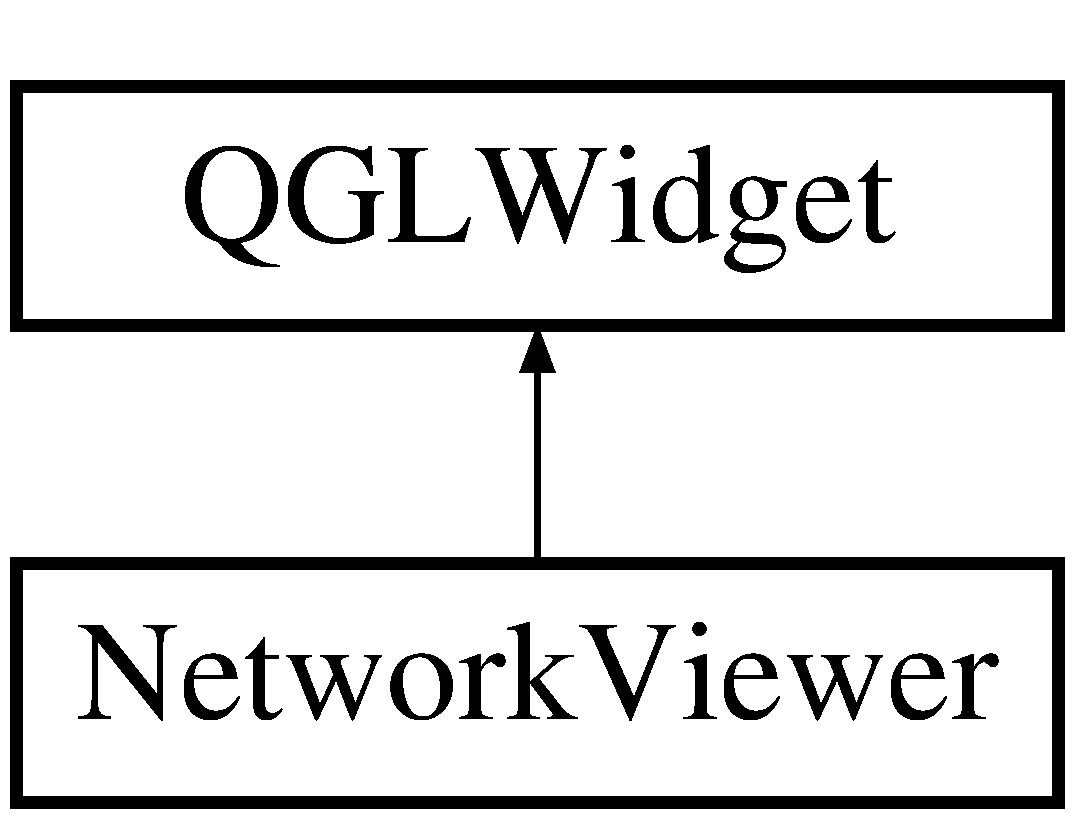
\includegraphics[height=2.000000cm]{classNetworkViewer}
\end{center}
\end{figure}
\subsection*{Public Member Functions}
\begin{DoxyCompactItemize}
\item 
\hypertarget{classNetworkViewer_aaf994e08d9ddf05c795762d093cf182b}{\hyperlink{classNetwork}{Network} $\ast$ {\bfseries get\-\_\-network} ()}\label{classNetworkViewer_aaf994e08d9ddf05c795762d093cf182b}

\item 
\hypertarget{classNetworkViewer_a0621900d2fe95a2a300875c8d0ff4c51}{{\bfseries Network\-Viewer} (\hyperlink{classNetwork}{Network} $\ast$network, Q\-Widget $\ast$parent=0, const Q\-G\-L\-Widget $\ast$share\-Widget=0, Qt\-::\-Window\-Flags f=0)}\label{classNetworkViewer_a0621900d2fe95a2a300875c8d0ff4c51}

\item 
\hypertarget{classNetworkViewer_aa2f63ab66d75cd2a380912d784982431}{void {\bfseries add\-\_\-view} (int x, int y, int width, int height)}\label{classNetworkViewer_aa2f63ab66d75cd2a380912d784982431}

\item 
\hypertarget{classNetworkViewer_ac46772e2b7880456c11b49b31c3f7ac3}{void {\bfseries split\-\_\-horizontally} (unsigned int view\-\_\-index=0, unsigned int width\-\_\-factor=2)}\label{classNetworkViewer_ac46772e2b7880456c11b49b31c3f7ac3}

\item 
\hypertarget{classNetworkViewer_aa9fa6833eca3a8ef7895899d7650a8d5}{void {\bfseries split\-\_\-vertically} (unsigned int view\-\_\-index=0, unsigned int height\-\_\-factor=2)}\label{classNetworkViewer_aa9fa6833eca3a8ef7895899d7650a8d5}

\item 
\hypertarget{classNetworkViewer_aee18b6c7626299d9d506f277e31f8d8a}{void {\bfseries home} (unsigned int index=0)}\label{classNetworkViewer_aee18b6c7626299d9d506f277e31f8d8a}

\item 
\hypertarget{classNetworkViewer_a6d5b973c63f14d0f7ae82458bcf0b8dc}{void {\bfseries forward} (double distance, unsigned int index=0)}\label{classNetworkViewer_a6d5b973c63f14d0f7ae82458bcf0b8dc}

\item 
\hypertarget{classNetworkViewer_a2ad8f6a1171116276c0b1ab4759d33d5}{void {\bfseries backward} (double distance, unsigned int index=0)}\label{classNetworkViewer_a2ad8f6a1171116276c0b1ab4759d33d5}

\item 
\hypertarget{classNetworkViewer_af9562ff09c492e8585949c81fc23d4ac}{void {\bfseries left} (double distance, unsigned int index=0)}\label{classNetworkViewer_af9562ff09c492e8585949c81fc23d4ac}

\item 
\hypertarget{classNetworkViewer_a5ed8a0eab674053dede6bc3067f43ac9}{void {\bfseries right} (double distance, unsigned int index=0)}\label{classNetworkViewer_a5ed8a0eab674053dede6bc3067f43ac9}

\item 
\hypertarget{classNetworkViewer_a0350eeac58d5853762a55aa805a790ae}{void {\bfseries up} (double distance, unsigned int index=0)}\label{classNetworkViewer_a0350eeac58d5853762a55aa805a790ae}

\item 
\hypertarget{classNetworkViewer_a4dc18dee6de49a7a882146d1dc042920}{void {\bfseries down} (double distance, unsigned int index=0)}\label{classNetworkViewer_a4dc18dee6de49a7a882146d1dc042920}

\item 
\hypertarget{classNetworkViewer_a68c39b3b90a5f3c847b6cc1c29ac1bdd}{void {\bfseries zoom} (double factor, unsigned int index=0)}\label{classNetworkViewer_a68c39b3b90a5f3c847b6cc1c29ac1bdd}

\item 
\hypertarget{classNetworkViewer_a52635efef221b6ad5c7d6b4e59f4f63e}{void {\bfseries roll} (double angle, unsigned int index=0)}\label{classNetworkViewer_a52635efef221b6ad5c7d6b4e59f4f63e}

\item 
\hypertarget{classNetworkViewer_a3ad896c71f1cac628029b621086fcc14}{void {\bfseries pitch} (double angle, unsigned int index=0)}\label{classNetworkViewer_a3ad896c71f1cac628029b621086fcc14}

\item 
\hypertarget{classNetworkViewer_aaa76f95495f6eac1861bd02d3fd7cfc6}{void {\bfseries yaw} (double angle, unsigned int index=0)}\label{classNetworkViewer_aaa76f95495f6eac1861bd02d3fd7cfc6}

\end{DoxyCompactItemize}
\subsection*{Public Attributes}
\begin{DoxyCompactItemize}
\item 
\hypertarget{classNetworkViewer_a3d87f11b2d01de7aad3efdb3f259ad6b}{double {\bfseries up\-\_\-distance}}\label{classNetworkViewer_a3d87f11b2d01de7aad3efdb3f259ad6b}

\item 
\hypertarget{classNetworkViewer_a904195fe44212c6d25baebfc13c9abcd}{double {\bfseries down\-\_\-distance}}\label{classNetworkViewer_a904195fe44212c6d25baebfc13c9abcd}

\item 
\hypertarget{classNetworkViewer_a9eb84b57a3f43ee8c13d1483f77b0aeb}{double {\bfseries left\-\_\-distance}}\label{classNetworkViewer_a9eb84b57a3f43ee8c13d1483f77b0aeb}

\item 
\hypertarget{classNetworkViewer_ab42043ac74e3ab946d10fa06e3789bc6}{double {\bfseries right\-\_\-distance}}\label{classNetworkViewer_ab42043ac74e3ab946d10fa06e3789bc6}

\item 
\hypertarget{classNetworkViewer_ab39b9b70d5a00215b1e674aeb502cc19}{double {\bfseries forward\-\_\-distance}}\label{classNetworkViewer_ab39b9b70d5a00215b1e674aeb502cc19}

\item 
\hypertarget{classNetworkViewer_a1f114369e408806185a04f35add06fd8}{double {\bfseries backward\-\_\-distance}}\label{classNetworkViewer_a1f114369e408806185a04f35add06fd8}

\item 
\hypertarget{classNetworkViewer_a08af11bdf6aa8c4d5ab7e838cd777aba}{double {\bfseries zoom\-\_\-factor}}\label{classNetworkViewer_a08af11bdf6aa8c4d5ab7e838cd777aba}

\item 
\hypertarget{classNetworkViewer_ac594ac2dffca4e5bb6484ace299b9083}{double {\bfseries roll\-\_\-angle}}\label{classNetworkViewer_ac594ac2dffca4e5bb6484ace299b9083}

\item 
\hypertarget{classNetworkViewer_a5463eae07405bab33fe4f9f9f78a20a4}{double {\bfseries pitch\-\_\-angle}}\label{classNetworkViewer_a5463eae07405bab33fe4f9f9f78a20a4}

\item 
\hypertarget{classNetworkViewer_ae94a3dd73d82e1b593eea0fa723a2470}{double {\bfseries yaw\-\_\-angle}}\label{classNetworkViewer_ae94a3dd73d82e1b593eea0fa723a2470}

\end{DoxyCompactItemize}
\subsection*{Protected Member Functions}
\begin{DoxyCompactItemize}
\item 
\hypertarget{classNetworkViewer_a17c4c12ad9a2fbda3594a9e78b4906cd}{virtual void {\bfseries paint\-Event} (Q\-Paint\-Event $\ast$paint\-Event)}\label{classNetworkViewer_a17c4c12ad9a2fbda3594a9e78b4906cd}

\item 
\hypertarget{classNetworkViewer_a2c49c3d3501e61ddddafbbfdcbcf5890}{virtual void {\bfseries paint\-G\-L} ()}\label{classNetworkViewer_a2c49c3d3501e61ddddafbbfdcbcf5890}

\item 
\hypertarget{classNetworkViewer_a01a40bdfbb3d4fa38ef733a5cdbdfce4}{virtual void {\bfseries resize\-G\-L} (int width, int height)}\label{classNetworkViewer_a01a40bdfbb3d4fa38ef733a5cdbdfce4}

\item 
\hypertarget{classNetworkViewer_a9002909ad3d5c9c380f8af24cc7dfda2}{virtual void {\bfseries key\-Press\-Event} (Q\-Key\-Event $\ast$event)}\label{classNetworkViewer_a9002909ad3d5c9c380f8af24cc7dfda2}

\item 
\hypertarget{classNetworkViewer_a72fd3375fadcecf5ef2d7659ae01e855}{virtual void {\bfseries key\-Release\-Event} (Q\-Key\-Event $\ast$event)}\label{classNetworkViewer_a72fd3375fadcecf5ef2d7659ae01e855}

\item 
\hypertarget{classNetworkViewer_a43a29c2847490d713ef6e67d64a69ec1}{virtual void {\bfseries mouse\-Move\-Event} (Q\-Mouse\-Event $\ast$event)}\label{classNetworkViewer_a43a29c2847490d713ef6e67d64a69ec1}

\item 
\hypertarget{classNetworkViewer_a5f6fe634093c6a84b6c7a17874a892d2}{virtual void {\bfseries mouse\-Press\-Event} (Q\-Mouse\-Event $\ast$event)}\label{classNetworkViewer_a5f6fe634093c6a84b6c7a17874a892d2}

\item 
\hypertarget{classNetworkViewer_a47bfd07665faf9ae2f666f5606e20645}{virtual void {\bfseries mouse\-Release\-Event} (Q\-Mouse\-Event $\ast$event)}\label{classNetworkViewer_a47bfd07665faf9ae2f666f5606e20645}

\item 
\hypertarget{classNetworkViewer_afae1fb278367ebcc033eabae20944e2f}{virtual void {\bfseries wheel\-Event} (Q\-Wheel\-Event $\ast$event)}\label{classNetworkViewer_afae1fb278367ebcc033eabae20944e2f}

\item 
\hypertarget{classNetworkViewer_aa85d947a8547b5de37f6022e578563f6}{virtual bool {\bfseries event} (Q\-Event $\ast$event)}\label{classNetworkViewer_aa85d947a8547b5de37f6022e578563f6}

\end{DoxyCompactItemize}


\subsection{Detailed Description}


Definition at line 10 of file Network\-Viewer.\-hpp.



The documentation for this class was generated from the following files\-:\begin{DoxyCompactItemize}
\item 
/home/aviral/\-Projects/moogli/moogli/include/view/Network\-Viewer.\-hpp\item 
/home/aviral/\-Projects/moogli/moogli/src/view/Network\-Viewer.\-cpp\end{DoxyCompactItemize}

\hypertarget{classNeuron}{\section{Neuron Class Reference}
\label{classNeuron}\index{Neuron@{Neuron}}
}
\subsection*{Public Member Functions}
\begin{DoxyCompactItemize}
\item 
\hypertarget{classNeuron_a700b5247c7dc30e35371f11027b71889}{{\bfseries Neuron} (const char $\ast$id)}\label{classNeuron_a700b5247c7dc30e35371f11027b71889}

\item 
\hypertarget{classNeuron_af9cb6fa1f5eebae02f76ac4708f32739}{const char $\ast$ {\bfseries get\-\_\-id} ()}\label{classNeuron_af9cb6fa1f5eebae02f76ac4708f32739}

\item 
\hypertarget{classNeuron_ad2f149ae34342bff4efa0e488554b802}{void {\bfseries set\-\_\-network} (\hyperlink{classNetwork}{Network} $\ast$network)}\label{classNeuron_ad2f149ae34342bff4efa0e488554b802}

\item 
\hypertarget{classNeuron_ad91b6fd7beb2cb35b82059e354983ea9}{\hyperlink{classNetwork}{Network} $\ast$ {\bfseries get\-\_\-network} ()}\label{classNeuron_ad91b6fd7beb2cb35b82059e354983ea9}

\item 
\hypertarget{classNeuron_afec51c42ecfc188d64181c10125ab458}{\hyperlink{classCompartment}{Compartment} $\ast$ {\bfseries get\-\_\-compartment} (const char $\ast$id)}\label{classNeuron_afec51c42ecfc188d64181c10125ab458}

\item 
\hypertarget{classNeuron_a0bca1dfb98292631f31734bbe6e54fe5}{void {\bfseries hide} ()}\label{classNeuron_a0bca1dfb98292631f31734bbe6e54fe5}

\item 
\hypertarget{classNeuron_af0e274af219c1d8f45cc511f5d761d2c}{void {\bfseries show} ()}\label{classNeuron_af0e274af219c1d8f45cc511f5d761d2c}

\item 
\hypertarget{classNeuron_aa6fe51d251379fb2514465024740dbd9}{bool {\bfseries is\-\_\-visible} ()}\label{classNeuron_aa6fe51d251379fb2514465024740dbd9}

\item 
\hypertarget{classNeuron_a4ebb973d49a16f4ee332c7b5d5c89d59}{unsigned int {\bfseries size} ()}\label{classNeuron_a4ebb973d49a16f4ee332c7b5d5c89d59}

\item 
\hypertarget{classNeuron_a878d0f990eb4aa2fd2827f228e7e1f74}{unsigned int {\bfseries add\-\_\-geometry} (Py\-Object $\ast$distal, Py\-Object $\ast$proximal=Py\-\_\-\-None, Py\-Object $\ast$parent=Py\-\_\-\-None)}\label{classNeuron_a878d0f990eb4aa2fd2827f228e7e1f74}

\item 
\hypertarget{classNeuron_a32adf0e61082065658c9d247b02b5e3b}{unsigned int {\bfseries add\-\_\-compartment} (\hyperlink{classCompartment}{Compartment} $\ast$compartment)}\label{classNeuron_a32adf0e61082065658c9d247b02b5e3b}

\item 
\hypertarget{classNeuron_ab46566c6c4b49375811d50502c716329}{unsigned int {\bfseries remove\-\_\-compartment} (\hyperlink{classCompartment}{Compartment} $\ast$compartment)}\label{classNeuron_ab46566c6c4b49375811d50502c716329}

\item 
\hypertarget{classNeuron_ab8784f82a6467442f2ddbb921e612ff2}{void {\bfseries show\-\_\-geometry} (unsigned int geometry\-\_\-index, bool hide\-\_\-others)}\label{classNeuron_ab8784f82a6467442f2ddbb921e612ff2}

\item 
\hypertarget{classNeuron_a623aa995b8b4f957272c6932e3986c09}{void {\bfseries hide\-\_\-geometry} (unsigned int geometry\-\_\-index)}\label{classNeuron_a623aa995b8b4f957272c6932e3986c09}

\item 
\hypertarget{classNeuron_a82af601b43aee10e772081d40481e90a}{void {\bfseries show\-\_\-all\-\_\-geometries} ()}\label{classNeuron_a82af601b43aee10e772081d40481e90a}

\item 
\hypertarget{classNeuron_a59ec3cae0be2e818de48494f14900e8b}{void {\bfseries hide\-\_\-all\-\_\-geometries} ()}\label{classNeuron_a59ec3cae0be2e818de48494f14900e8b}

\item 
\hypertarget{classNeuron_a1062ac27f56bf9212b2f2e7a0a9c7fcf}{void {\bfseries set\-\_\-color} (Py\-Object $\ast$color)}\label{classNeuron_a1062ac27f56bf9212b2f2e7a0a9c7fcf}

\item 
\hypertarget{classNeuron_ae4e41149b9251116a407227388640552}{bool {\bfseries set\-\_\-colors} (Py\-Object $\ast$colors)}\label{classNeuron_ae4e41149b9251116a407227388640552}

\end{DoxyCompactItemize}
\subsection*{Public Attributes}
\begin{DoxyCompactItemize}
\item 
\hypertarget{classNeuron_a1c503e02c29f6b5c8a1840a6e0a847e3}{string {\bfseries id}}\label{classNeuron_a1c503e02c29f6b5c8a1840a6e0a847e3}

\item 
\hypertarget{classNeuron_af4bdb3f8cf8632347adb3eeec89537e1}{\hyperlink{classNetwork}{Network} $\ast$ {\bfseries network}}\label{classNeuron_af4bdb3f8cf8632347adb3eeec89537e1}

\item 
\hypertarget{classNeuron_a56ba863d9204d9e962889cbcb1ff2181}{osg\-::ref\-\_\-ptr$<$ osg\-::\-Switch $>$ {\bfseries node}}\label{classNeuron_a56ba863d9204d9e962889cbcb1ff2181}

\item 
\hypertarget{classNeuron_a0af3d6fb2d7f69e85ee9d6ac50bd31bc}{osg\-::ref\-\_\-ptr$<$ osg\-::\-Group $>$ {\bfseries compartment\-\_\-group\-\_\-node}}\label{classNeuron_a0af3d6fb2d7f69e85ee9d6ac50bd31bc}

\item 
\hypertarget{classNeuron_a6d30e48d2a4d43a65d0f904e12db7d1f}{std\-::vector$<$ \hyperlink{classCompartment}{Compartment} $\ast$ $>$ {\bfseries compartment\-\_\-seq}}\label{classNeuron_a6d30e48d2a4d43a65d0f904e12db7d1f}

\item 
\hypertarget{classNeuron_a30d03e58657a0383b3298ca220ae5d4a}{std\-::unordered\-\_\-map$<$ string, \\*
\hyperlink{classCompartment}{Compartment} $\ast$ $>$ {\bfseries compartment\-\_\-map}}\label{classNeuron_a30d03e58657a0383b3298ca220ae5d4a}

\end{DoxyCompactItemize}


\subsection{Detailed Description}


Definition at line 10 of file Neuron.\-hpp.



The documentation for this class was generated from the following files\-:\begin{DoxyCompactItemize}
\item 
/home/aviral/\-Projects/moogli/moogli/include/core/Neuron.\-hpp\item 
/home/aviral/\-Projects/moogli/moogli/src/core/Neuron.\-cpp\end{DoxyCompactItemize}

\hypertarget{classpoint_1_1Point}{\section{point.\-Point Class Reference}
\label{classpoint_1_1Point}\index{point.\-Point@{point.\-Point}}
}
\subsection*{Public Member Functions}
\begin{DoxyCompactItemize}
\item 
\hypertarget{classpoint_1_1Point_a4f2882f4c1d41b8ed0dcc040a56df10e}{def {\bfseries \-\_\-\-\_\-init\-\_\-\-\_\-}}\label{classpoint_1_1Point_a4f2882f4c1d41b8ed0dcc040a56df10e}

\item 
\hypertarget{classpoint_1_1Point_a1ae81c5e1d69b5ccac1e489a798eff70}{def {\bfseries \-\_\-\-\_\-str\-\_\-\-\_\-}}\label{classpoint_1_1Point_a1ae81c5e1d69b5ccac1e489a798eff70}

\item 
\hypertarget{classpoint_1_1Point_aace59f3313d86fffb9315171d1f68440}{def {\bfseries \-\_\-\-\_\-add\-\_\-\-\_\-}}\label{classpoint_1_1Point_aace59f3313d86fffb9315171d1f68440}

\item 
\hypertarget{classpoint_1_1Point_a63d6c9a6aaf7b41618ff8b18336eb6bd}{def {\bfseries \-\_\-\-\_\-sub\-\_\-\-\_\-}}\label{classpoint_1_1Point_a63d6c9a6aaf7b41618ff8b18336eb6bd}

\item 
\hypertarget{classpoint_1_1Point_a4c61f633eea69f44555e8d42852cbfbc}{def {\bfseries \-\_\-\-\_\-rmul\-\_\-\-\_\-}}\label{classpoint_1_1Point_a4c61f633eea69f44555e8d42852cbfbc}

\item 
\hypertarget{classpoint_1_1Point_a74924a7729713d7115462c3390e0cba8}{def {\bfseries \-\_\-\-\_\-div\-\_\-\-\_\-}}\label{classpoint_1_1Point_a74924a7729713d7115462c3390e0cba8}

\item 
\hypertarget{classpoint_1_1Point_a63cbb86ade8b1aade58afd232fa6625f}{def {\bfseries \-\_\-\-\_\-xor\-\_\-\-\_\-}}\label{classpoint_1_1Point_a63cbb86ade8b1aade58afd232fa6625f}

\item 
\hypertarget{classpoint_1_1Point_a89e9195409206f59e74e34e16cb1176e}{def {\bfseries \-\_\-\-\_\-pow\-\_\-\-\_\-}}\label{classpoint_1_1Point_a89e9195409206f59e74e34e16cb1176e}

\item 
\hypertarget{classpoint_1_1Point_a14147c8780809dc0c0e040c95ed0222a}{def {\bfseries magnitude}}\label{classpoint_1_1Point_a14147c8780809dc0c0e040c95ed0222a}

\item 
\hypertarget{classpoint_1_1Point_ae4ef371493c544fb0c74ec8e65a533af}{def {\bfseries normalize}}\label{classpoint_1_1Point_ae4ef371493c544fb0c74ec8e65a533af}

\end{DoxyCompactItemize}
\subsection*{Public Attributes}
\begin{DoxyCompactItemize}
\item 
\hypertarget{classpoint_1_1Point_a8ad40c4544ff2978d58c89abdb34d607}{{\bfseries x}}\label{classpoint_1_1Point_a8ad40c4544ff2978d58c89abdb34d607}

\item 
\hypertarget{classpoint_1_1Point_a353d1b0ca4635fd6d6e85ad9a7633710}{{\bfseries y}}\label{classpoint_1_1Point_a353d1b0ca4635fd6d6e85ad9a7633710}

\item 
\hypertarget{classpoint_1_1Point_a7c0bcd0bef9336ea208f3fa06746a8b7}{{\bfseries z}}\label{classpoint_1_1Point_a7c0bcd0bef9336ea208f3fa06746a8b7}

\end{DoxyCompactItemize}


\subsection{Detailed Description}


The documentation for this class was generated from the following file\-:\begin{DoxyCompactItemize}
\item 
/home/aviral/\-Projects/moogli/moogli/geometry/point.\-py\end{DoxyCompactItemize}

\hypertarget{classSphereMesh}{\section{Sphere\-Mesh Class Reference}
\label{classSphereMesh}\index{Sphere\-Mesh@{Sphere\-Mesh}}
}
\subsection*{Public Member Functions}
\begin{DoxyCompactItemize}
\item 
\hypertarget{classSphereMesh_ac2f74a159e2c440e570fcc96eccd3bc7}{Geometry $\ast$ {\bfseries operator()} (Vec3f center, float radius, unsigned int points, const Vec4 \&color)}\label{classSphereMesh_ac2f74a159e2c440e570fcc96eccd3bc7}

\item 
\hypertarget{classSphereMesh_a8b27a3b7b6bfbe78ef36f10b45be3674}{void {\bfseries operator()} (Vec3f center, float radius, Geometry $\ast$geometry, unsigned int points, const Vec4 \&color)}\label{classSphereMesh_a8b27a3b7b6bfbe78ef36f10b45be3674}

\end{DoxyCompactItemize}


\subsection{Detailed Description}


Definition at line 30 of file Sphere\-Mesh.\-hpp.



The documentation for this class was generated from the following files\-:\begin{DoxyCompactItemize}
\item 
/home/aviral/\-Projects/moogli/moogli/include/mesh/Sphere\-Mesh.\-hpp\item 
/home/aviral/\-Projects/moogli/moogli/src/mesh/Sphere\-Mesh.\-cpp\end{DoxyCompactItemize}

\hypertarget{classVoxel}{\section{Voxel Class Reference}
\label{classVoxel}\index{Voxel@{Voxel}}
}
\subsection*{Public Member Functions}
\begin{DoxyCompactItemize}
\item 
\hypertarget{classVoxel_a8d82b79d00ae9f6029605d312ab178c7}{{\bfseries Voxel} (const char $\ast$id)}\label{classVoxel_a8d82b79d00ae9f6029605d312ab178c7}

\item 
\hypertarget{classVoxel_a08eb8268674f69f5d6187fe0a89a8158}{const char $\ast$ {\bfseries get\-\_\-id} ()}\label{classVoxel_a08eb8268674f69f5d6187fe0a89a8158}

\item 
\hypertarget{classVoxel_aebd6e95739e95b440cc08d62ce7ce96b}{void {\bfseries set\-\_\-compartment} (\hyperlink{classCompartment}{Compartment} $\ast$compartment)}\label{classVoxel_aebd6e95739e95b440cc08d62ce7ce96b}

\item 
\hypertarget{classVoxel_ab125a4817085bda442ae22713c1d898c}{\hyperlink{classCompartment}{Compartment} $\ast$ {\bfseries get\-\_\-compartment} ()}\label{classVoxel_ab125a4817085bda442ae22713c1d898c}

\item 
\hypertarget{classVoxel_a8d78a6c3090d280ad18647e0152fd8e1}{void {\bfseries hide} ()}\label{classVoxel_a8d78a6c3090d280ad18647e0152fd8e1}

\item 
\hypertarget{classVoxel_a27b81d57c913bb25de47499de667ee0e}{void {\bfseries show} ()}\label{classVoxel_a27b81d57c913bb25de47499de667ee0e}

\item 
\hypertarget{classVoxel_afa7b4f931236036eb814431c45972502}{bool {\bfseries is\-\_\-visible} ()}\label{classVoxel_afa7b4f931236036eb814431c45972502}

\item 
\hypertarget{classVoxel_a045e38b04d04e42ef2ec80de1101f261}{void {\bfseries set\-\_\-geometry} (Py\-Object $\ast$distal, Py\-Object $\ast$proximal=Py\-\_\-\-None, Py\-Object $\ast$parent=Py\-\_\-\-None)}\label{classVoxel_a045e38b04d04e42ef2ec80de1101f261}

\item 
\hypertarget{classVoxel_ad71dda7683ac7ca9f19c286eee3a4fc8}{void {\bfseries set\-\_\-color} (Py\-Object $\ast$color)}\label{classVoxel_ad71dda7683ac7ca9f19c286eee3a4fc8}

\end{DoxyCompactItemize}
\subsection*{Public Attributes}
\begin{DoxyCompactItemize}
\item 
\hypertarget{classVoxel_a29721ad4b3ba72ffdaf0858ceb59f1d8}{string {\bfseries id}}\label{classVoxel_a29721ad4b3ba72ffdaf0858ceb59f1d8}

\item 
\hypertarget{classVoxel_ab2e89f3ae2c8df9aa1a2b0822bdada06}{\hyperlink{classCompartment}{Compartment} $\ast$ {\bfseries compartment}}\label{classVoxel_ab2e89f3ae2c8df9aa1a2b0822bdada06}

\item 
\hypertarget{classVoxel_ac88e6ca57921bfd8e9cfe3d997d3b780}{osg\-::ref\-\_\-ptr$<$ osg\-::\-Geometry $>$ {\bfseries node}}\label{classVoxel_ac88e6ca57921bfd8e9cfe3d997d3b780}

\end{DoxyCompactItemize}


\subsection{Detailed Description}


Definition at line 8 of file Voxel.\-hpp.



The documentation for this class was generated from the following files\-:\begin{DoxyCompactItemize}
\item 
/home/aviral/\-Projects/moogli/moogli/include/core/Voxel.\-hpp\item 
/home/aviral/\-Projects/moogli/moogli/src/core/Voxel.\-cpp\end{DoxyCompactItemize}

%--- End generated contents ---

% Index
\newpage
\phantomsection
\addcontentsline{toc}{chapter}{Index}
\printindex

\end{document}
